% Created by tikzDevice version 0.12 on 2019-05-20 15:24:33
% !TEX encoding = UTF-8 Unicode
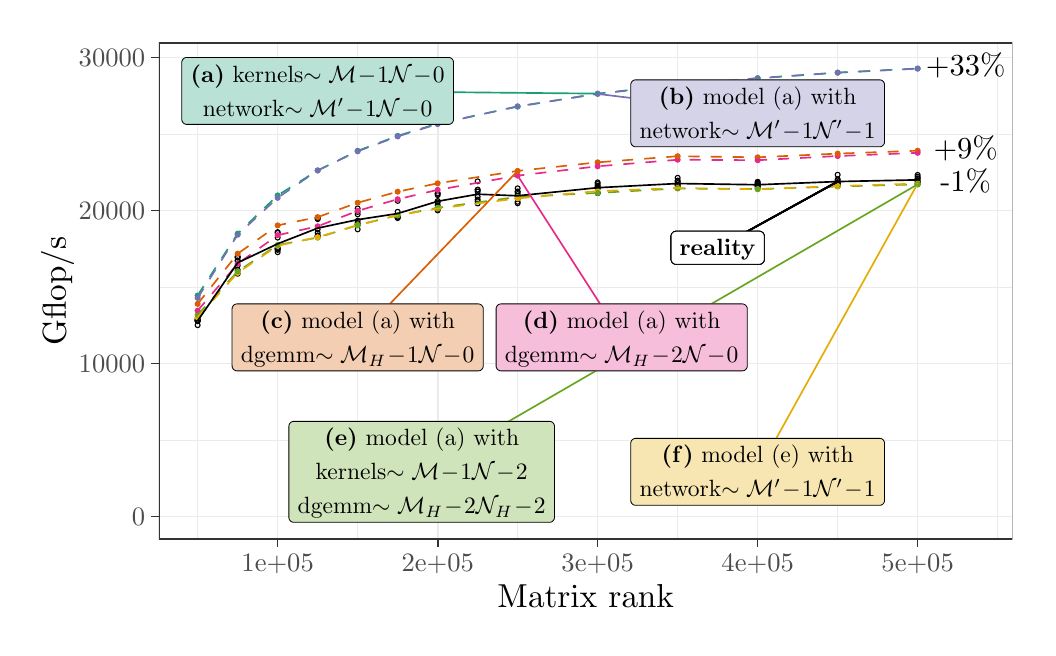
\begin{tikzpicture}[x=1pt,y=1pt]
\definecolor{fillColor}{RGB}{255,255,255}
\path[use as bounding box,fill=fillColor,fill opacity=0.00] (0,0) rectangle (361.35,216.81);
\begin{scope}
\path[clip] (  0.00,  0.00) rectangle (361.35,216.81);
\definecolor{drawColor}{RGB}{255,255,255}
\definecolor{fillColor}{RGB}{255,255,255}

\path[draw=drawColor,line width= 0.6pt,line join=round,line cap=round,fill=fillColor] (  0.00,  0.00) rectangle (361.35,216.81);
\end{scope}
\begin{scope}
\path[clip] ( 47.40, 31.96) rectangle (355.85,211.31);
\definecolor{fillColor}{RGB}{255,255,255}

\path[fill=fillColor] ( 47.40, 31.96) rectangle (355.85,211.31);
\definecolor{drawColor}{gray}{0.92}

\path[draw=drawColor,line width= 0.3pt,line join=round] ( 47.40, 67.77) --
	(355.85, 67.77);

\path[draw=drawColor,line width= 0.3pt,line join=round] ( 47.40,123.08) --
	(355.85,123.08);

\path[draw=drawColor,line width= 0.3pt,line join=round] ( 47.40,178.38) --
	(355.85,178.38);

\path[draw=drawColor,line width= 0.3pt,line join=round] ( 61.42, 31.96) --
	( 61.42,211.31);

\path[draw=drawColor,line width= 0.3pt,line join=round] (119.24, 31.96) --
	(119.24,211.31);

\path[draw=drawColor,line width= 0.3pt,line join=round] (177.05, 31.96) --
	(177.05,211.31);

\path[draw=drawColor,line width= 0.3pt,line join=round] (234.87, 31.96) --
	(234.87,211.31);

\path[draw=drawColor,line width= 0.3pt,line join=round] (292.69, 31.96) --
	(292.69,211.31);

\path[draw=drawColor,line width= 0.3pt,line join=round] (350.50, 31.96) --
	(350.50,211.31);

\path[draw=drawColor,line width= 0.6pt,line join=round] ( 47.40, 40.12) --
	(355.85, 40.12);

\path[draw=drawColor,line width= 0.6pt,line join=round] ( 47.40, 95.42) --
	(355.85, 95.42);

\path[draw=drawColor,line width= 0.6pt,line join=round] ( 47.40,150.73) --
	(355.85,150.73);

\path[draw=drawColor,line width= 0.6pt,line join=round] ( 47.40,206.03) --
	(355.85,206.03);

\path[draw=drawColor,line width= 0.6pt,line join=round] ( 90.33, 31.96) --
	( 90.33,211.31);

\path[draw=drawColor,line width= 0.6pt,line join=round] (148.15, 31.96) --
	(148.15,211.31);

\path[draw=drawColor,line width= 0.6pt,line join=round] (205.96, 31.96) --
	(205.96,211.31);

\path[draw=drawColor,line width= 0.6pt,line join=round] (263.78, 31.96) --
	(263.78,211.31);

\path[draw=drawColor,line width= 0.6pt,line join=round] (321.59, 31.96) --
	(321.59,211.31);
\definecolor{drawColor}{RGB}{0,0,0}

\path[draw=drawColor,line width= 0.4pt,line join=round,line cap=round] (321.59,163.61) circle (  0.89);

\path[draw=drawColor,line width= 0.4pt,line join=round,line cap=round] ( 61.42,110.80) circle (  0.89);

\path[draw=drawColor,line width= 0.4pt,line join=round,line cap=round] (205.96,157.03) circle (  0.89);

\path[draw=drawColor,line width= 0.4pt,line join=round,line cap=round] (263.78,159.91) circle (  0.89);

\path[draw=drawColor,line width= 0.4pt,line join=round,line cap=round] (119.24,150.23) circle (  0.89);

\path[draw=drawColor,line width= 0.4pt,line join=round,line cap=round] (177.05,153.88) circle (  0.89);

\path[draw=drawColor,line width= 0.4pt,line join=round,line cap=round] (292.69,162.01) circle (  0.89);

\path[draw=drawColor,line width= 0.4pt,line join=round,line cap=round] (234.87,162.56) circle (  0.89);

\path[draw=drawColor,line width= 0.4pt,line join=round,line cap=round] (148.15,154.16) circle (  0.89);

\path[draw=drawColor,line width= 0.4pt,line join=round,line cap=round] ( 90.33,142.65) circle (  0.89);

\path[draw=drawColor,line width= 0.4pt,line join=round,line cap=round] ( 75.88,134.08) circle (  0.89);

\path[draw=drawColor,line width= 0.4pt,line join=round,line cap=round] (104.79,147.63) circle (  0.89);

\path[draw=drawColor,line width= 0.4pt,line join=round,line cap=round] (162.60,158.30) circle (  0.89);

\path[draw=drawColor,line width= 0.4pt,line join=round,line cap=round] ( 75.88,133.92) circle (  0.89);

\path[draw=drawColor,line width= 0.4pt,line join=round,line cap=round] (205.96,160.90) circle (  0.89);

\path[draw=drawColor,line width= 0.4pt,line join=round,line cap=round] (292.69,163.67) circle (  0.89);

\path[draw=drawColor,line width= 0.4pt,line join=round,line cap=round] (148.15,156.98) circle (  0.89);

\path[draw=drawColor,line width= 0.4pt,line join=round,line cap=round] (133.69,148.18) circle (  0.89);

\path[draw=drawColor,line width= 0.4pt,line join=round,line cap=round] ( 61.42,110.85) circle (  0.89);

\path[draw=drawColor,line width= 0.4pt,line join=round,line cap=round] (162.60,161.29) circle (  0.89);

\path[draw=drawColor,line width= 0.4pt,line join=round,line cap=round] (177.05,157.64) circle (  0.89);

\path[draw=drawColor,line width= 0.4pt,line join=round,line cap=round] (104.79,141.44) circle (  0.89);

\path[draw=drawColor,line width= 0.4pt,line join=round,line cap=round] (119.24,147.08) circle (  0.89);

\path[draw=drawColor,line width= 0.4pt,line join=round,line cap=round] ( 90.33,142.93) circle (  0.89);

\path[draw=drawColor,line width= 0.4pt,line join=round,line cap=round] (321.59,162.40) circle (  0.89);

\path[draw=drawColor,line width= 0.4pt,line join=round,line cap=round] (263.78,161.13) circle (  0.89);

\path[draw=drawColor,line width= 0.4pt,line join=round,line cap=round] (234.87,159.08) circle (  0.89);

\path[draw=drawColor,line width= 0.4pt,line join=round,line cap=round] ( 61.42,111.13) circle (  0.89);

\path[draw=drawColor,line width= 0.4pt,line join=round,line cap=round] (104.79,141.27) circle (  0.89);

\path[draw=drawColor,line width= 0.4pt,line join=round,line cap=round] (321.59,160.57) circle (  0.89);

\path[draw=drawColor,line width= 0.4pt,line join=round,line cap=round] (162.60,154.10) circle (  0.89);

\path[draw=drawColor,line width= 0.4pt,line join=round,line cap=round] (119.24,149.35) circle (  0.89);

\path[draw=drawColor,line width= 0.4pt,line join=round,line cap=round] (263.78,160.35) circle (  0.89);

\path[draw=drawColor,line width= 0.4pt,line join=round,line cap=round] ( 75.88,129.27) circle (  0.89);

\path[draw=drawColor,line width= 0.4pt,line join=round,line cap=round] (205.96,158.80) circle (  0.89);

\path[draw=drawColor,line width= 0.4pt,line join=round,line cap=round] (234.87,160.63) circle (  0.89);

\path[draw=drawColor,line width= 0.4pt,line join=round,line cap=round] (292.69,161.62) circle (  0.89);

\path[draw=drawColor,line width= 0.4pt,line join=round,line cap=round] (177.05,154.99) circle (  0.89);

\path[draw=drawColor,line width= 0.4pt,line join=round,line cap=round] (148.15,156.31) circle (  0.89);

\path[draw=drawColor,line width= 0.4pt,line join=round,line cap=round] ( 90.33,136.51) circle (  0.89);

\path[draw=drawColor,line width= 0.4pt,line join=round,line cap=round] (133.69,148.46) circle (  0.89);

\path[draw=drawColor,line width= 0.4pt,line join=round,line cap=round] (177.05,156.70) circle (  0.89);

\path[draw=drawColor,line width= 0.4pt,line join=round,line cap=round] ( 61.42,109.30) circle (  0.89);

\path[draw=drawColor,line width= 0.4pt,line join=round,line cap=round] (205.96,158.75) circle (  0.89);

\path[draw=drawColor,line width= 0.4pt,line join=round,line cap=round] (104.79,141.77) circle (  0.89);

\path[draw=drawColor,line width= 0.4pt,line join=round,line cap=round] ( 90.33,137.23) circle (  0.89);

\path[draw=drawColor,line width= 0.4pt,line join=round,line cap=round] (321.59,162.95) circle (  0.89);

\path[draw=drawColor,line width= 0.4pt,line join=round,line cap=round] ( 75.88,132.70) circle (  0.89);

\path[draw=drawColor,line width= 0.4pt,line join=round,line cap=round] (119.24,145.70) circle (  0.89);

\path[draw=drawColor,line width= 0.4pt,line join=round,line cap=round] (148.15,153.66) circle (  0.89);

\path[draw=drawColor,line width= 0.4pt,line join=round,line cap=round] (263.78,160.35) circle (  0.89);

\path[draw=drawColor,line width= 0.4pt,line join=round,line cap=round] (162.60,155.71) circle (  0.89);

\path[draw=drawColor,line width= 0.4pt,line join=round,line cap=round] (292.69,159.74) circle (  0.89);

\path[draw=drawColor,line width= 0.4pt,line join=round,line cap=round] (133.69,148.68) circle (  0.89);

\path[draw=drawColor,line width= 0.4pt,line join=round,line cap=round] (234.87,160.02) circle (  0.89);

\path[draw=drawColor,line width= 0.4pt,line join=round,line cap=round] (148.15,151.28) circle (  0.89);

\path[draw=drawColor,line width= 0.4pt,line join=round,line cap=round] (292.69,160.57) circle (  0.89);

\path[draw=drawColor,line width= 0.4pt,line join=round,line cap=round] (133.69,150.29) circle (  0.89);

\path[draw=drawColor,line width= 0.4pt,line join=round,line cap=round] (263.78,158.80) circle (  0.89);

\path[draw=drawColor,line width= 0.4pt,line join=round,line cap=round] (177.05,155.82) circle (  0.89);

\path[draw=drawColor,line width= 0.4pt,line join=round,line cap=round] ( 61.42,111.79) circle (  0.89);

\path[draw=drawColor,line width= 0.4pt,line join=round,line cap=round] (205.96,159.19) circle (  0.89);

\path[draw=drawColor,line width= 0.4pt,line join=round,line cap=round] (321.59,160.24) circle (  0.89);

\path[draw=drawColor,line width= 0.4pt,line join=round,line cap=round] ( 75.88,133.69) circle (  0.89);

\path[draw=drawColor,line width= 0.4pt,line join=round,line cap=round] (104.79,148.07) circle (  0.89);

\path[draw=drawColor,line width= 0.4pt,line join=round,line cap=round] (119.24,151.50) circle (  0.89);

\path[draw=drawColor,line width= 0.4pt,line join=round,line cap=round] ( 90.33,135.68) circle (  0.89);

\path[draw=drawColor,line width= 0.4pt,line join=round,line cap=round] (162.60,154.71) circle (  0.89);

\path[draw=drawColor,line width= 0.4pt,line join=round,line cap=round] (234.87,158.91) circle (  0.89);

\path[draw=drawColor,line width= 0.4pt,line join=round,line cap=round] (321.59,161.13) circle (  0.89);

\path[draw=drawColor,line width= 0.4pt,line join=round,line cap=round] ( 61.42,110.91) circle (  0.89);

\path[draw=drawColor,line width= 0.4pt,line join=round,line cap=round] (205.96,157.09) circle (  0.89);

\path[draw=drawColor,line width= 0.4pt,line join=round,line cap=round] (263.78,159.69) circle (  0.89);

\path[draw=drawColor,line width= 0.4pt,line join=round,line cap=round] (119.24,146.19) circle (  0.89);

\path[draw=drawColor,line width= 0.4pt,line join=round,line cap=round] (177.05,157.36) circle (  0.89);

\path[draw=drawColor,line width= 0.4pt,line join=round,line cap=round] (292.69,160.63) circle (  0.89);

\path[draw=drawColor,line width= 0.4pt,line join=round,line cap=round] (234.87,159.91) circle (  0.89);

\path[draw=drawColor,line width= 0.4pt,line join=round,line cap=round] (148.15,150.78) circle (  0.89);

\path[draw=drawColor,line width= 0.4pt,line join=round,line cap=round] ( 90.33,136.79) circle (  0.89);

\path[draw=drawColor,line width= 0.4pt,line join=round,line cap=round] ( 75.88,130.82) circle (  0.89);

\path[draw=drawColor,line width= 0.4pt,line join=round,line cap=round] (104.79,148.13) circle (  0.89);

\path[draw=drawColor,line width= 0.4pt,line join=round,line cap=round] (162.60,157.53) circle (  0.89);

\path[draw=drawColor,line width= 0.4pt,line join=round,line cap=round] ( 75.88,127.89) circle (  0.89);

\path[draw=drawColor,line width= 0.4pt,line join=round,line cap=round] (205.96,160.35) circle (  0.89);

\path[draw=drawColor,line width= 0.4pt,line join=round,line cap=round] (292.69,160.35) circle (  0.89);

\path[draw=drawColor,line width= 0.4pt,line join=round,line cap=round] (148.15,152.61) circle (  0.89);

\path[draw=drawColor,line width= 0.4pt,line join=round,line cap=round] (133.69,154.21) circle (  0.89);

\path[draw=drawColor,line width= 0.4pt,line join=round,line cap=round] ( 61.42,111.13) circle (  0.89);

\path[draw=drawColor,line width= 0.4pt,line join=round,line cap=round] (162.60,153.27) circle (  0.89);

\path[draw=drawColor,line width= 0.4pt,line join=round,line cap=round] (177.05,153.33) circle (  0.89);

\path[draw=drawColor,line width= 0.4pt,line join=round,line cap=round] (104.79,143.98) circle (  0.89);

\path[draw=drawColor,line width= 0.4pt,line join=round,line cap=round] (119.24,143.93) circle (  0.89);

\path[draw=drawColor,line width= 0.4pt,line join=round,line cap=round] ( 90.33,136.90) circle (  0.89);

\path[draw=drawColor,line width= 0.4pt,line join=round,line cap=round] (321.59,161.40) circle (  0.89);

\path[draw=drawColor,line width= 0.4pt,line join=round,line cap=round] (263.78,160.79) circle (  0.89);

\path[draw=drawColor,line width= 0.4pt,line join=round,line cap=round] (234.87,161.24) circle (  0.89);

\path[draw=drawColor,line width= 0.4pt,line join=round,line cap=round] ( 61.42,111.24) circle (  0.89);

\path[draw=drawColor,line width= 0.4pt,line join=round,line cap=round] (104.79,142.71) circle (  0.89);

\path[draw=drawColor,line width= 0.4pt,line join=round,line cap=round] (321.59,162.18) circle (  0.89);

\path[draw=drawColor,line width= 0.4pt,line join=round,line cap=round] (162.60,158.14) circle (  0.89);

\path[draw=drawColor,line width= 0.4pt,line join=round,line cap=round] (119.24,145.47) circle (  0.89);

\path[draw=drawColor,line width= 0.4pt,line join=round,line cap=round] (263.78,159.41) circle (  0.89);

\path[draw=drawColor,line width= 0.4pt,line join=round,line cap=round] ( 75.88,132.53) circle (  0.89);

\path[draw=drawColor,line width= 0.4pt,line join=round,line cap=round] (205.96,159.69) circle (  0.89);

\path[draw=drawColor,line width= 0.4pt,line join=round,line cap=round] (234.87,161.57) circle (  0.89);

\path[draw=drawColor,line width= 0.4pt,line join=round,line cap=round] (292.69,161.01) circle (  0.89);

\path[draw=drawColor,line width= 0.4pt,line join=round,line cap=round] (177.05,158.75) circle (  0.89);

\path[draw=drawColor,line width= 0.4pt,line join=round,line cap=round] (148.15,156.76) circle (  0.89);

\path[draw=drawColor,line width= 0.4pt,line join=round,line cap=round] ( 90.33,140.94) circle (  0.89);

\path[draw=drawColor,line width= 0.4pt,line join=round,line cap=round] (133.69,148.02) circle (  0.89);
\definecolor{drawColor}{RGB}{230,171,2}
\definecolor{fillColor}{RGB}{230,171,2}

\path[draw=drawColor,line width= 0.4pt,line join=round,line cap=round,fill=fillColor] ( 75.88,128.22) circle (  0.89);

\path[draw=drawColor,line width= 0.4pt,line join=round,line cap=round,fill=fillColor] (133.69,149.01) circle (  0.89);

\path[draw=drawColor,line width= 0.4pt,line join=round,line cap=round,fill=fillColor] (234.87,158.86) circle (  0.89);
\definecolor{drawColor}{RGB}{217,95,2}
\definecolor{fillColor}{RGB}{217,95,2}

\path[draw=drawColor,line width= 0.4pt,line join=round,line cap=round,fill=fillColor] ( 61.42,116.99) circle (  0.89);

\path[draw=drawColor,line width= 0.4pt,line join=round,line cap=round,fill=fillColor] (119.24,153.55) circle (  0.89);

\path[draw=drawColor,line width= 0.4pt,line join=round,line cap=round,fill=fillColor] (205.96,168.15) circle (  0.89);

\path[draw=drawColor,line width= 0.4pt,line join=round,line cap=round,fill=fillColor] (321.59,172.35) circle (  0.89);
\definecolor{drawColor}{RGB}{230,171,2}
\definecolor{fillColor}{RGB}{230,171,2}

\path[draw=drawColor,line width= 0.4pt,line join=round,line cap=round,fill=fillColor] ( 90.33,138.01) circle (  0.89);

\path[draw=drawColor,line width= 0.4pt,line join=round,line cap=round,fill=fillColor] (148.15,151.45) circle (  0.89);

\path[draw=drawColor,line width= 0.4pt,line join=round,line cap=round,fill=fillColor] (263.78,158.42) circle (  0.89);

\path[draw=drawColor,line width= 0.4pt,line join=round,line cap=round,fill=fillColor] ( 61.42,112.12) circle (  0.89);

\path[draw=drawColor,line width= 0.4pt,line join=round,line cap=round,fill=fillColor] (119.24,145.47) circle (  0.89);

\path[draw=drawColor,line width= 0.4pt,line join=round,line cap=round,fill=fillColor] (205.96,157.75) circle (  0.89);

\path[draw=drawColor,line width= 0.4pt,line join=round,line cap=round,fill=fillColor] (321.59,160.46) circle (  0.89);
\definecolor{drawColor}{RGB}{231,41,138}
\definecolor{fillColor}{RGB}{231,41,138}

\path[draw=drawColor,line width= 0.4pt,line join=round,line cap=round,fill=fillColor] ( 75.88,131.48) circle (  0.89);

\path[draw=drawColor,line width= 0.4pt,line join=round,line cap=round,fill=fillColor] (133.69,154.82) circle (  0.89);

\path[draw=drawColor,line width= 0.4pt,line join=round,line cap=round,fill=fillColor] (234.87,169.09) circle (  0.89);
\definecolor{drawColor}{RGB}{102,166,30}
\definecolor{fillColor}{RGB}{102,166,30}

\path[draw=drawColor,line width= 0.4pt,line join=round,line cap=round,fill=fillColor] ( 61.42,113.06) circle (  0.89);

\path[draw=drawColor,line width= 0.4pt,line join=round,line cap=round,fill=fillColor] (119.24,145.42) circle (  0.89);

\path[draw=drawColor,line width= 0.4pt,line join=round,line cap=round,fill=fillColor] (205.96,157.09) circle (  0.89);

\path[draw=drawColor,line width= 0.4pt,line join=round,line cap=round,fill=fillColor] (321.59,160.19) circle (  0.89);
\definecolor{drawColor}{RGB}{231,41,138}
\definecolor{fillColor}{RGB}{231,41,138}

\path[draw=drawColor,line width= 0.4pt,line join=round,line cap=round,fill=fillColor] ( 61.42,114.56) circle (  0.89);

\path[draw=drawColor,line width= 0.4pt,line join=round,line cap=round,fill=fillColor] (119.24,150.62) circle (  0.89);

\path[draw=drawColor,line width= 0.4pt,line join=round,line cap=round,fill=fillColor] (205.96,166.71) circle (  0.89);

\path[draw=drawColor,line width= 0.4pt,line join=round,line cap=round,fill=fillColor] (321.59,171.58) circle (  0.89);

\path[draw=drawColor,line width= 0.4pt,line join=round,line cap=round,fill=fillColor] (104.79,145.03) circle (  0.89);

\path[draw=drawColor,line width= 0.4pt,line join=round,line cap=round,fill=fillColor] (177.05,163.34) circle (  0.89);

\path[draw=drawColor,line width= 0.4pt,line join=round,line cap=round,fill=fillColor] (292.69,170.42) circle (  0.89);
\definecolor{drawColor}{RGB}{217,95,2}
\definecolor{fillColor}{RGB}{217,95,2}

\path[draw=drawColor,line width= 0.4pt,line join=round,line cap=round,fill=fillColor] ( 75.88,135.13) circle (  0.89);

\path[draw=drawColor,line width= 0.4pt,line join=round,line cap=round,fill=fillColor] (133.69,157.53) circle (  0.89);

\path[draw=drawColor,line width= 0.4pt,line join=round,line cap=round,fill=fillColor] (234.87,170.36) circle (  0.89);

\path[draw=drawColor,line width= 0.4pt,line join=round,line cap=round,fill=fillColor] (104.79,148.35) circle (  0.89);

\path[draw=drawColor,line width= 0.4pt,line join=round,line cap=round,fill=fillColor] (177.05,165.05) circle (  0.89);

\path[draw=drawColor,line width= 0.4pt,line join=round,line cap=round,fill=fillColor] (292.69,171.30) circle (  0.89);
\definecolor{drawColor}{RGB}{102,166,30}
\definecolor{fillColor}{RGB}{102,166,30}

\path[draw=drawColor,line width= 0.4pt,line join=round,line cap=round,fill=fillColor] (104.79,140.94) circle (  0.89);

\path[draw=drawColor,line width= 0.4pt,line join=round,line cap=round,fill=fillColor] (177.05,155.65) circle (  0.89);

\path[draw=drawColor,line width= 0.4pt,line join=round,line cap=round,fill=fillColor] (292.69,159.41) circle (  0.89);
\definecolor{drawColor}{RGB}{230,171,2}
\definecolor{fillColor}{RGB}{230,171,2}

\path[draw=drawColor,line width= 0.4pt,line join=round,line cap=round,fill=fillColor] (104.79,141.10) circle (  0.89);

\path[draw=drawColor,line width= 0.4pt,line join=round,line cap=round,fill=fillColor] (177.05,155.10) circle (  0.89);

\path[draw=drawColor,line width= 0.4pt,line join=round,line cap=round,fill=fillColor] (292.69,159.58) circle (  0.89);
\definecolor{drawColor}{RGB}{102,166,30}
\definecolor{fillColor}{RGB}{102,166,30}

\path[draw=drawColor,line width= 0.4pt,line join=round,line cap=round,fill=fillColor] ( 75.88,128.72) circle (  0.89);

\path[draw=drawColor,line width= 0.4pt,line join=round,line cap=round,fill=fillColor] (133.69,149.01) circle (  0.89);

\path[draw=drawColor,line width= 0.4pt,line join=round,line cap=round,fill=fillColor] (234.87,158.69) circle (  0.89);

\path[draw=drawColor,line width= 0.4pt,line join=round,line cap=round,fill=fillColor] ( 90.33,138.28) circle (  0.89);

\path[draw=drawColor,line width= 0.4pt,line join=round,line cap=round,fill=fillColor] (148.15,151.72) circle (  0.89);

\path[draw=drawColor,line width= 0.4pt,line join=round,line cap=round,fill=fillColor] (263.78,158.47) circle (  0.89);
\definecolor{drawColor}{RGB}{217,95,2}
\definecolor{fillColor}{RGB}{217,95,2}

\path[draw=drawColor,line width= 0.4pt,line join=round,line cap=round,fill=fillColor] ( 90.33,145.36) circle (  0.89);

\path[draw=drawColor,line width= 0.4pt,line join=round,line cap=round,fill=fillColor] (148.15,160.57) circle (  0.89);

\path[draw=drawColor,line width= 0.4pt,line join=round,line cap=round,fill=fillColor] (263.78,169.97) circle (  0.89);
\definecolor{drawColor}{RGB}{231,41,138}
\definecolor{fillColor}{RGB}{231,41,138}

\path[draw=drawColor,line width= 0.4pt,line join=round,line cap=round,fill=fillColor] ( 90.33,141.82) circle (  0.89);

\path[draw=drawColor,line width= 0.4pt,line join=round,line cap=round,fill=fillColor] (148.15,158.19) circle (  0.89);

\path[draw=drawColor,line width= 0.4pt,line join=round,line cap=round,fill=fillColor] (263.78,168.92) circle (  0.89);
\definecolor{drawColor}{RGB}{27,158,119}
\definecolor{fillColor}{RGB}{27,158,119}

\path[draw=drawColor,line width= 0.4pt,line join=round,line cap=round,fill=fillColor] (321.59,202.05) circle (  0.89);

\path[draw=drawColor,line width= 0.4pt,line join=round,line cap=round,fill=fillColor] ( 61.42,120.03) circle (  0.89);

\path[draw=drawColor,line width= 0.4pt,line join=round,line cap=round,fill=fillColor] (205.96,192.98) circle (  0.89);

\path[draw=drawColor,line width= 0.4pt,line join=round,line cap=round,fill=fillColor] (263.78,198.57) circle (  0.89);

\path[draw=drawColor,line width= 0.4pt,line join=round,line cap=round,fill=fillColor] (119.24,172.30) circle (  0.89);

\path[draw=drawColor,line width= 0.4pt,line join=round,line cap=round,fill=fillColor] (148.15,182.14) circle (  0.89);

\path[draw=drawColor,line width= 0.4pt,line join=round,line cap=round,fill=fillColor] ( 90.33,156.20) circle (  0.89);

\path[draw=drawColor,line width= 0.4pt,line join=round,line cap=round,fill=fillColor] (133.69,177.72) circle (  0.89);

\path[draw=drawColor,line width= 0.4pt,line join=round,line cap=round,fill=fillColor] (177.05,188.28) circle (  0.89);

\path[draw=drawColor,line width= 0.4pt,line join=round,line cap=round,fill=fillColor] (292.69,200.56) circle (  0.89);

\path[draw=drawColor,line width= 0.4pt,line join=round,line cap=round,fill=fillColor] (234.87,196.19) circle (  0.89);

\path[draw=drawColor,line width= 0.4pt,line join=round,line cap=round,fill=fillColor] ( 75.88,142.38) circle (  0.89);

\path[draw=drawColor,line width= 0.4pt,line join=round,line cap=round,fill=fillColor] (104.79,165.22) circle (  0.89);
\definecolor{drawColor}{RGB}{117,112,179}
\definecolor{fillColor}{RGB}{117,112,179}

\path[draw=drawColor,line width= 0.4pt,line join=round,line cap=round,fill=fillColor] (321.59,202.00) circle (  0.89);

\path[draw=drawColor,line width= 0.4pt,line join=round,line cap=round,fill=fillColor] ( 61.42,119.15) circle (  0.89);

\path[draw=drawColor,line width= 0.4pt,line join=round,line cap=round,fill=fillColor] (205.96,192.87) circle (  0.89);

\path[draw=drawColor,line width= 0.4pt,line join=round,line cap=round,fill=fillColor] (263.78,198.51) circle (  0.89);

\path[draw=drawColor,line width= 0.4pt,line join=round,line cap=round,fill=fillColor] (119.24,172.13) circle (  0.89);

\path[draw=drawColor,line width= 0.4pt,line join=round,line cap=round,fill=fillColor] (148.15,181.98) circle (  0.89);

\path[draw=drawColor,line width= 0.4pt,line join=round,line cap=round,fill=fillColor] ( 90.33,155.32) circle (  0.89);

\path[draw=drawColor,line width= 0.4pt,line join=round,line cap=round,fill=fillColor] (133.69,177.50) circle (  0.89);

\path[draw=drawColor,line width= 0.4pt,line join=round,line cap=round,fill=fillColor] (177.05,188.39) circle (  0.89);

\path[draw=drawColor,line width= 0.4pt,line join=round,line cap=round,fill=fillColor] (292.69,200.56) circle (  0.89);

\path[draw=drawColor,line width= 0.4pt,line join=round,line cap=round,fill=fillColor] (234.87,196.13) circle (  0.89);

\path[draw=drawColor,line width= 0.4pt,line join=round,line cap=round,fill=fillColor] ( 75.88,141.99) circle (  0.89);

\path[draw=drawColor,line width= 0.4pt,line join=round,line cap=round,fill=fillColor] (104.79,165.22) circle (  0.89);
\definecolor{drawColor}{RGB}{27,158,119}

\path[draw=drawColor,line width= 0.6pt,dash pattern=on 4pt off 4pt ,line join=round] ( 61.42,120.03) --
	( 75.88,142.38) --
	( 90.33,156.20) --
	(104.79,165.22) --
	(119.24,172.30) --
	(133.69,177.72) --
	(148.15,182.14) --
	(177.05,188.28) --
	(205.96,192.98) --
	(234.87,196.19) --
	(263.78,198.57) --
	(292.69,200.56) --
	(321.59,202.05);
\definecolor{drawColor}{RGB}{217,95,2}

\path[draw=drawColor,line width= 0.6pt,dash pattern=on 4pt off 4pt ,line join=round] ( 61.42,116.99) --
	( 75.88,135.13) --
	( 90.33,145.36) --
	(104.79,148.35) --
	(119.24,153.55) --
	(133.69,157.53) --
	(148.15,160.57) --
	(177.05,165.05) --
	(205.96,168.15) --
	(234.87,170.36) --
	(263.78,169.97) --
	(292.69,171.30) --
	(321.59,172.35);
\definecolor{drawColor}{RGB}{117,112,179}

\path[draw=drawColor,line width= 0.6pt,dash pattern=on 4pt off 4pt ,line join=round] ( 61.42,119.15) --
	( 75.88,141.99) --
	( 90.33,155.32) --
	(104.79,165.22) --
	(119.24,172.13) --
	(133.69,177.50) --
	(148.15,181.98) --
	(177.05,188.39) --
	(205.96,192.87) --
	(234.87,196.13) --
	(263.78,198.51) --
	(292.69,200.56) --
	(321.59,202.00);
\definecolor{drawColor}{RGB}{231,41,138}

\path[draw=drawColor,line width= 0.6pt,dash pattern=on 4pt off 4pt ,line join=round] ( 61.42,114.56) --
	( 75.88,131.48) --
	( 90.33,141.82) --
	(104.79,145.03) --
	(119.24,150.62) --
	(133.69,154.82) --
	(148.15,158.19) --
	(177.05,163.34) --
	(205.96,166.71) --
	(234.87,169.09) --
	(263.78,168.92) --
	(292.69,170.42) --
	(321.59,171.58);
\definecolor{drawColor}{RGB}{102,166,30}

\path[draw=drawColor,line width= 0.6pt,dash pattern=on 4pt off 4pt ,line join=round] ( 61.42,113.06) --
	( 75.88,128.72) --
	( 90.33,138.28) --
	(104.79,140.94) --
	(119.24,145.42) --
	(133.69,149.01) --
	(148.15,151.72) --
	(177.05,155.65) --
	(205.96,157.09) --
	(234.87,158.69) --
	(263.78,158.47) --
	(292.69,159.41) --
	(321.59,160.19);
\definecolor{drawColor}{RGB}{230,171,2}

\path[draw=drawColor,line width= 0.6pt,dash pattern=on 4pt off 4pt ,line join=round] ( 61.42,112.12) --
	( 75.88,128.22) --
	( 90.33,138.01) --
	(104.79,141.10) --
	(119.24,145.47) --
	(133.69,149.01) --
	(148.15,151.45) --
	(177.05,155.10) --
	(205.96,157.75) --
	(234.87,158.86) --
	(263.78,158.42) --
	(292.69,159.58) --
	(321.59,160.46);
\definecolor{drawColor}{RGB}{0,0,0}

\path[draw=drawColor,line width= 0.6pt,line join=round] ( 61.42,110.89) --
	( 75.88,131.86) --
	( 90.33,138.71) --
	(104.79,144.37) --
	(119.24,147.43) --
	(133.69,149.64) --
	(148.15,154.07) --
	(162.60,156.63) --
	(177.05,156.06) --
	(205.96,158.98) --
	(234.87,160.49) --
	(263.78,160.05) --
	(292.69,161.20) --
	(321.59,161.81);
\definecolor{drawColor}{RGB}{230,171,2}

\path[draw=drawColor,line width= 0.6pt,line join=round] (263.78, 56.31) -- (321.59,160.46);
\definecolor{drawColor}{RGB}{102,166,30}

\path[draw=drawColor,line width= 0.6pt,line join=round] (142.37, 56.31) -- (321.59,160.19);
\definecolor{drawColor}{RGB}{231,41,138}

\path[draw=drawColor,line width= 0.6pt,line join=round] (214.63,104.89) -- (177.05,163.34);
\definecolor{drawColor}{RGB}{217,95,2}

\path[draw=drawColor,line width= 0.6pt,line join=round] (119.24,104.89) -- (177.05,165.05);
\definecolor{drawColor}{RGB}{27,158,119}

\path[draw=drawColor,line width= 0.6pt,line join=round] (104.79,193.96) -- (205.96,192.98);
\definecolor{drawColor}{RGB}{117,112,179}

\path[draw=drawColor,line width= 0.6pt,line join=round] (263.78,185.86) -- (205.96,192.87);
\definecolor{drawColor}{RGB}{255,255,255}
\definecolor{fillColor}{RGB}{255,255,255}

\path[draw=drawColor,line width= 0.3pt,line join=round,line cap=round,fill=fillColor] (219.73, 44.21) --
	(307.82, 44.21) --
	(307.75, 44.21) --
	(308.04, 44.23) --
	(308.33, 44.28) --
	(308.60, 44.39) --
	(308.85, 44.53) --
	(309.07, 44.72) --
	(309.27, 44.93) --
	(309.42, 45.18) --
	(309.54, 45.45) --
	(309.61, 45.73) --
	(309.63, 46.02) --
	(309.63, 46.02) --
	(309.63, 66.60) --
	(309.63, 66.60) --
	(309.61, 66.89) --
	(309.54, 67.17) --
	(309.42, 67.44) --
	(309.27, 67.69) --
	(309.07, 67.90) --
	(308.85, 68.09) --
	(308.60, 68.23) --
	(308.33, 68.34) --
	(308.04, 68.39) --
	(307.82, 68.41) --
	(219.73, 68.41) --
	(219.95, 68.39) --
	(219.66, 68.41) --
	(219.37, 68.37) --
	(219.09, 68.29) --
	(218.83, 68.16) --
	(218.59, 68.00) --
	(218.38, 67.80) --
	(218.21, 67.57) --
	(218.07, 67.31) --
	(217.98, 67.03) --
	(217.93, 66.75) --
	(217.93, 66.60) --
	(217.93, 46.02) --
	(217.93, 46.17) --
	(217.93, 45.87) --
	(217.98, 45.59) --
	(218.07, 45.31) --
	(218.21, 45.05) --
	(218.38, 44.82) --
	(218.59, 44.62) --
	(218.83, 44.46) --
	(219.09, 44.33) --
	(219.37, 44.25) --
	(219.66, 44.21) --
	cycle;
\end{scope}
\begin{scope}
\path[clip] ( 47.40, 31.96) rectangle (355.85,211.31);
\definecolor{drawColor}{RGB}{255,255,255}

\node[text=drawColor,anchor=base,inner sep=0pt, outer sep=0pt, scale=  0.85] at (263.78, 59.52) {\textbf{(f)} model (e) with};

\node[text=drawColor,anchor=base,inner sep=0pt, outer sep=0pt, scale=  0.85] at (263.78, 47.22) {network$\sim\mathcal{M'}\!-\!1 \mathcal{N'}\!-\!1$};
\definecolor{fillColor}{RGB}{255,255,255}

\path[draw=drawColor,line width= 0.3pt,line join=round,line cap=round,fill=fillColor] ( 96.19, 38.07) --
	(188.54, 38.07) --
	(188.47, 38.07) --
	(188.76, 38.08) --
	(189.05, 38.14) --
	(189.32, 38.24) --
	(189.57, 38.39) --
	(189.80, 38.57) --
	(189.99, 38.79) --
	(190.14, 39.03) --
	(190.26, 39.30) --
	(190.33, 39.58) --
	(190.35, 39.87) --
	(190.35, 39.87) --
	(190.35, 72.75) --
	(190.35, 72.75) --
	(190.33, 73.04) --
	(190.26, 73.32) --
	(190.14, 73.59) --
	(189.99, 73.83) --
	(189.80, 74.05) --
	(189.57, 74.23) --
	(189.32, 74.38) --
	(189.05, 74.48) --
	(188.76, 74.54) --
	(188.54, 74.55) --
	( 96.19, 74.55) --
	( 96.40, 74.54) --
	( 96.11, 74.55) --
	( 95.82, 74.52) --
	( 95.55, 74.43) --
	( 95.28, 74.31) --
	( 95.04, 74.15) --
	( 94.83, 73.94) --
	( 94.66, 73.71) --
	( 94.52, 73.45) --
	( 94.43, 73.18) --
	( 94.39, 72.89) --
	( 94.38, 72.75) --
	( 94.38, 39.87) --
	( 94.39, 40.02) --
	( 94.39, 39.73) --
	( 94.43, 39.44) --
	( 94.52, 39.17) --
	( 94.66, 38.91) --
	( 94.83, 38.68) --
	( 95.04, 38.47) --
	( 95.28, 38.31) --
	( 95.55, 38.19) --
	( 95.82, 38.10) --
	( 96.11, 38.07) --
	cycle;
\end{scope}
\begin{scope}
\path[clip] ( 47.40, 31.96) rectangle (355.85,211.31);
\definecolor{drawColor}{RGB}{255,255,255}

\node[text=drawColor,anchor=base,inner sep=0pt, outer sep=0pt, scale=  0.85] at (142.37, 65.66) {\textbf{(e)} model (a) with};

\node[text=drawColor,anchor=base,inner sep=0pt, outer sep=0pt, scale=  0.85] at (142.37, 53.37) {kernels$\sim\mathcal{M}\!-\!1 \mathcal{N}\!-\!2$};

\node[text=drawColor,anchor=base,inner sep=0pt, outer sep=0pt, scale=  0.85] at (142.37, 41.08) {dgemm$\sim\mathcal{M}_{H}\!-\!2 \mathcal{N}_{H}\!-\!2$};
\definecolor{fillColor}{RGB}{255,255,255}

\path[draw=drawColor,line width= 0.3pt,line join=round,line cap=round,fill=fillColor] (171.06, 92.79) --
	(258.21, 92.79) --
	(258.13, 92.80) --
	(258.42, 92.81) --
	(258.71, 92.87) --
	(258.98, 92.97) --
	(259.23, 93.11) --
	(259.46, 93.30) --
	(259.65, 93.52) --
	(259.81, 93.76) --
	(259.92, 94.03) --
	(259.99, 94.31) --
	(260.01, 94.60) --
	(260.01, 94.60) --
	(260.01,115.18) --
	(260.01,115.18) --
	(259.99,115.47) --
	(259.92,115.75) --
	(259.81,116.02) --
	(259.65,116.27) --
	(259.46,116.48) --
	(259.23,116.67) --
	(258.98,116.81) --
	(258.71,116.92) --
	(258.42,116.97) --
	(258.21,116.99) --
	(171.06,116.99) --
	(171.28,116.97) --
	(170.99,116.99) --
	(170.70,116.95) --
	(170.42,116.87) --
	(170.16,116.75) --
	(169.92,116.58) --
	(169.71,116.38) --
	(169.54,116.15) --
	(169.40,115.89) --
	(169.31,115.61) --
	(169.26,115.33) --
	(169.26,115.18) --
	(169.26, 94.60) --
	(169.26, 94.75) --
	(169.26, 94.46) --
	(169.31, 94.17) --
	(169.40, 93.89) --
	(169.54, 93.64) --
	(169.71, 93.40) --
	(169.92, 93.20) --
	(170.16, 93.04) --
	(170.42, 92.91) --
	(170.70, 92.83) --
	(170.99, 92.80) --
	cycle;
\end{scope}
\begin{scope}
\path[clip] ( 47.40, 31.96) rectangle (355.85,211.31);
\definecolor{drawColor}{RGB}{255,255,255}

\node[text=drawColor,anchor=base,inner sep=0pt, outer sep=0pt, scale=  0.85] at (214.63,108.10) {\textbf{(d)} model (a) with};

\node[text=drawColor,anchor=base,inner sep=0pt, outer sep=0pt, scale=  0.85] at (214.63, 95.81) {dgemm$\sim\mathcal{M}_{H}\!-\!2 \mathcal{N}\!-\!0$};
\definecolor{fillColor}{RGB}{255,255,255}

\path[draw=drawColor,line width= 0.3pt,line join=round,line cap=round,fill=fillColor] ( 75.67, 92.79) --
	(162.81, 92.79) --
	(162.74, 92.80) --
	(163.03, 92.81) --
	(163.31, 92.87) --
	(163.58, 92.97) --
	(163.84, 93.11) --
	(164.06, 93.30) --
	(164.25, 93.52) --
	(164.41, 93.76) --
	(164.52, 94.03) --
	(164.59, 94.31) --
	(164.62, 94.60) --
	(164.62, 94.60) --
	(164.62,115.18) --
	(164.62,115.18) --
	(164.59,115.47) --
	(164.52,115.75) --
	(164.41,116.02) --
	(164.25,116.27) --
	(164.06,116.48) --
	(163.84,116.67) --
	(163.58,116.81) --
	(163.31,116.92) --
	(163.03,116.97) --
	(162.81,116.99) --
	( 75.67,116.99) --
	( 75.89,116.97) --
	( 75.60,116.99) --
	( 75.31,116.95) --
	( 75.03,116.87) --
	( 74.76,116.75) --
	( 74.53,116.58) --
	( 74.32,116.38) --
	( 74.14,116.15) --
	( 74.01,115.89) --
	( 73.91,115.61) --
	( 73.87,115.33) --
	( 73.86,115.18) --
	( 73.86, 94.60) --
	( 73.87, 94.75) --
	( 73.87, 94.46) --
	( 73.91, 94.17) --
	( 74.01, 93.89) --
	( 74.14, 93.64) --
	( 74.32, 93.40) --
	( 74.53, 93.20) --
	( 74.76, 93.04) --
	( 75.03, 92.91) --
	( 75.31, 92.83) --
	( 75.60, 92.80) --
	cycle;
\end{scope}
\begin{scope}
\path[clip] ( 47.40, 31.96) rectangle (355.85,211.31);
\definecolor{drawColor}{RGB}{255,255,255}

\node[text=drawColor,anchor=base,inner sep=0pt, outer sep=0pt, scale=  0.85] at (119.24,108.10) {\textbf{(c)} model (a) with};

\node[text=drawColor,anchor=base,inner sep=0pt, outer sep=0pt, scale=  0.85] at (119.24, 95.81) {dgemm$\sim\mathcal{M}_{H}\!-\!1 \mathcal{N}\!-\!0$};
\definecolor{fillColor}{RGB}{255,255,255}

\path[draw=drawColor,line width= 0.3pt,line join=round,line cap=round,fill=fillColor] ( 57.50,181.86) --
	(152.07,181.86) --
	(151.99,181.86) --
	(152.29,181.87) --
	(152.57,181.93) --
	(152.84,182.03) --
	(153.09,182.18) --
	(153.32,182.36) --
	(153.51,182.58) --
	(153.67,182.83) --
	(153.78,183.09) --
	(153.85,183.38) --
	(153.87,183.67) --
	(153.87,183.67) --
	(153.87,204.24) --
	(153.87,204.24) --
	(153.85,204.53) --
	(153.78,204.82) --
	(153.67,205.08) --
	(153.51,205.33) --
	(153.32,205.55) --
	(153.09,205.73) --
	(152.84,205.88) --
	(152.57,205.98) --
	(152.29,206.04) --
	(152.07,206.05) --
	( 57.50,206.05) --
	( 57.72,206.04) --
	( 57.43,206.05) --
	( 57.14,206.02) --
	( 56.86,205.93) --
	( 56.60,205.81) --
	( 56.36,205.64) --
	( 56.15,205.44) --
	( 55.98,205.21) --
	( 55.84,204.95) --
	( 55.75,204.68) --
	( 55.70,204.39) --
	( 55.70,204.24) --
	( 55.70,183.67) --
	( 55.70,183.81) --
	( 55.70,183.52) --
	( 55.75,183.23) --
	( 55.84,182.96) --
	( 55.98,182.70) --
	( 56.15,182.47) --
	( 56.36,182.27) --
	( 56.60,182.10) --
	( 56.86,181.98) --
	( 57.14,181.90) --
	( 57.43,181.86) --
	cycle;
\end{scope}
\begin{scope}
\path[clip] ( 47.40, 31.96) rectangle (355.85,211.31);
\definecolor{drawColor}{RGB}{255,255,255}

\node[text=drawColor,anchor=base,inner sep=0pt, outer sep=0pt, scale=  0.85] at (104.79,197.16) {\textbf{(a)} kernels$\sim\mathcal{M}\!-\!1 \mathcal{N}\!-\!0$};

\node[text=drawColor,anchor=base,inner sep=0pt, outer sep=0pt, scale=  0.85] at (104.79,184.87) {network$\sim\mathcal{M'}\!-\!1 \mathcal{N}\!-\!0$};
\definecolor{fillColor}{RGB}{255,255,255}

\path[draw=drawColor,line width= 0.3pt,line join=round,line cap=round,fill=fillColor] (219.73,173.76) --
	(307.82,173.76) --
	(307.75,173.76) --
	(308.04,173.77) --
	(308.33,173.83) --
	(308.60,173.94) --
	(308.85,174.08) --
	(309.07,174.27) --
	(309.27,174.48) --
	(309.42,174.73) --
	(309.54,175.00) --
	(309.61,175.28) --
	(309.63,175.57) --
	(309.63,175.57) --
	(309.63,196.15) --
	(309.63,196.15) --
	(309.61,196.44) --
	(309.54,196.72) --
	(309.42,196.99) --
	(309.27,197.23) --
	(309.07,197.45) --
	(308.85,197.63) --
	(308.60,197.78) --
	(308.33,197.88) --
	(308.04,197.94) --
	(307.82,197.95) --
	(219.73,197.95) --
	(219.95,197.94) --
	(219.66,197.95) --
	(219.37,197.92) --
	(219.09,197.84) --
	(218.83,197.71) --
	(218.59,197.55) --
	(218.38,197.35) --
	(218.21,197.11) --
	(218.07,196.86) --
	(217.98,196.58) --
	(217.93,196.29) --
	(217.93,196.15) --
	(217.93,175.57) --
	(217.93,175.71) --
	(217.93,175.42) --
	(217.98,175.14) --
	(218.07,174.86) --
	(218.21,174.60) --
	(218.38,174.37) --
	(218.59,174.17) --
	(218.83,174.00) --
	(219.09,173.88) --
	(219.37,173.80) --
	(219.66,173.76) --
	cycle;
\end{scope}
\begin{scope}
\path[clip] ( 47.40, 31.96) rectangle (355.85,211.31);
\definecolor{drawColor}{RGB}{255,255,255}

\node[text=drawColor,anchor=base,inner sep=0pt, outer sep=0pt, scale=  0.85] at (263.78,189.06) {\textbf{(b)} model (a) with};

\node[text=drawColor,anchor=base,inner sep=0pt, outer sep=0pt, scale=  0.85] at (263.78,176.77) {network$\sim\mathcal{M'}\!-\!1 \mathcal{N'}\!-\!1$};
\definecolor{drawColor}{RGB}{0,0,0}
\definecolor{fillColor}{RGB}{230,171,2}

\path[draw=drawColor,line width= 0.3pt,line join=round,line cap=round,fill=fillColor,fill opacity=0.30] (219.73, 44.21) --
	(307.82, 44.21) --
	(307.75, 44.21) --
	(308.04, 44.23) --
	(308.33, 44.28) --
	(308.60, 44.39) --
	(308.85, 44.53) --
	(309.07, 44.72) --
	(309.27, 44.93) --
	(309.42, 45.18) --
	(309.54, 45.45) --
	(309.61, 45.73) --
	(309.63, 46.02) --
	(309.63, 46.02) --
	(309.63, 66.60) --
	(309.63, 66.60) --
	(309.61, 66.89) --
	(309.54, 67.17) --
	(309.42, 67.44) --
	(309.27, 67.69) --
	(309.07, 67.90) --
	(308.85, 68.09) --
	(308.60, 68.23) --
	(308.33, 68.34) --
	(308.04, 68.39) --
	(307.82, 68.41) --
	(219.73, 68.41) --
	(219.95, 68.39) --
	(219.66, 68.41) --
	(219.37, 68.37) --
	(219.09, 68.29) --
	(218.83, 68.16) --
	(218.59, 68.00) --
	(218.38, 67.80) --
	(218.21, 67.57) --
	(218.07, 67.31) --
	(217.98, 67.03) --
	(217.93, 66.75) --
	(217.93, 66.60) --
	(217.93, 46.02) --
	(217.93, 46.17) --
	(217.93, 45.87) --
	(217.98, 45.59) --
	(218.07, 45.31) --
	(218.21, 45.05) --
	(218.38, 44.82) --
	(218.59, 44.62) --
	(218.83, 44.46) --
	(219.09, 44.33) --
	(219.37, 44.25) --
	(219.66, 44.21) --
	cycle;
\end{scope}
\begin{scope}
\path[clip] ( 47.40, 31.96) rectangle (355.85,211.31);
\definecolor{drawColor}{RGB}{0,0,0}

\node[text=drawColor,anchor=base,inner sep=0pt, outer sep=0pt, scale=  0.85] at (263.78, 59.52) {\textbf{(f)} model (e) with};

\node[text=drawColor,anchor=base,inner sep=0pt, outer sep=0pt, scale=  0.85] at (263.78, 47.22) {network$\sim\mathcal{M'}\!-\!1 \mathcal{N'}\!-\!1$};
\definecolor{fillColor}{RGB}{102,166,30}

\path[draw=drawColor,line width= 0.3pt,line join=round,line cap=round,fill=fillColor,fill opacity=0.30] ( 96.19, 38.07) --
	(188.54, 38.07) --
	(188.47, 38.07) --
	(188.76, 38.08) --
	(189.05, 38.14) --
	(189.32, 38.24) --
	(189.57, 38.39) --
	(189.80, 38.57) --
	(189.99, 38.79) --
	(190.14, 39.03) --
	(190.26, 39.30) --
	(190.33, 39.58) --
	(190.35, 39.87) --
	(190.35, 39.87) --
	(190.35, 72.75) --
	(190.35, 72.75) --
	(190.33, 73.04) --
	(190.26, 73.32) --
	(190.14, 73.59) --
	(189.99, 73.83) --
	(189.80, 74.05) --
	(189.57, 74.23) --
	(189.32, 74.38) --
	(189.05, 74.48) --
	(188.76, 74.54) --
	(188.54, 74.55) --
	( 96.19, 74.55) --
	( 96.40, 74.54) --
	( 96.11, 74.55) --
	( 95.82, 74.52) --
	( 95.55, 74.43) --
	( 95.28, 74.31) --
	( 95.04, 74.15) --
	( 94.83, 73.94) --
	( 94.66, 73.71) --
	( 94.52, 73.45) --
	( 94.43, 73.18) --
	( 94.39, 72.89) --
	( 94.38, 72.75) --
	( 94.38, 39.87) --
	( 94.39, 40.02) --
	( 94.39, 39.73) --
	( 94.43, 39.44) --
	( 94.52, 39.17) --
	( 94.66, 38.91) --
	( 94.83, 38.68) --
	( 95.04, 38.47) --
	( 95.28, 38.31) --
	( 95.55, 38.19) --
	( 95.82, 38.10) --
	( 96.11, 38.07) --
	cycle;
\end{scope}
\begin{scope}
\path[clip] ( 47.40, 31.96) rectangle (355.85,211.31);
\definecolor{drawColor}{RGB}{0,0,0}

\node[text=drawColor,anchor=base,inner sep=0pt, outer sep=0pt, scale=  0.85] at (142.37, 65.66) {\textbf{(e)} model (a) with};

\node[text=drawColor,anchor=base,inner sep=0pt, outer sep=0pt, scale=  0.85] at (142.37, 53.37) {kernels$\sim\mathcal{M}\!-\!1 \mathcal{N}\!-\!2$};

\node[text=drawColor,anchor=base,inner sep=0pt, outer sep=0pt, scale=  0.85] at (142.37, 41.08) {dgemm$\sim\mathcal{M}_{H}\!-\!2 \mathcal{N}_{H}\!-\!2$};
\definecolor{fillColor}{RGB}{231,41,138}

\path[draw=drawColor,line width= 0.3pt,line join=round,line cap=round,fill=fillColor,fill opacity=0.30] (171.06, 92.79) --
	(258.21, 92.79) --
	(258.13, 92.80) --
	(258.42, 92.81) --
	(258.71, 92.87) --
	(258.98, 92.97) --
	(259.23, 93.11) --
	(259.46, 93.30) --
	(259.65, 93.52) --
	(259.81, 93.76) --
	(259.92, 94.03) --
	(259.99, 94.31) --
	(260.01, 94.60) --
	(260.01, 94.60) --
	(260.01,115.18) --
	(260.01,115.18) --
	(259.99,115.47) --
	(259.92,115.75) --
	(259.81,116.02) --
	(259.65,116.27) --
	(259.46,116.48) --
	(259.23,116.67) --
	(258.98,116.81) --
	(258.71,116.92) --
	(258.42,116.97) --
	(258.21,116.99) --
	(171.06,116.99) --
	(171.28,116.97) --
	(170.99,116.99) --
	(170.70,116.95) --
	(170.42,116.87) --
	(170.16,116.75) --
	(169.92,116.58) --
	(169.71,116.38) --
	(169.54,116.15) --
	(169.40,115.89) --
	(169.31,115.61) --
	(169.26,115.33) --
	(169.26,115.18) --
	(169.26, 94.60) --
	(169.26, 94.75) --
	(169.26, 94.46) --
	(169.31, 94.17) --
	(169.40, 93.89) --
	(169.54, 93.64) --
	(169.71, 93.40) --
	(169.92, 93.20) --
	(170.16, 93.04) --
	(170.42, 92.91) --
	(170.70, 92.83) --
	(170.99, 92.80) --
	cycle;
\end{scope}
\begin{scope}
\path[clip] ( 47.40, 31.96) rectangle (355.85,211.31);
\definecolor{drawColor}{RGB}{0,0,0}

\node[text=drawColor,anchor=base,inner sep=0pt, outer sep=0pt, scale=  0.85] at (214.63,108.10) {\textbf{(d)} model (a) with};

\node[text=drawColor,anchor=base,inner sep=0pt, outer sep=0pt, scale=  0.85] at (214.63, 95.81) {dgemm$\sim\mathcal{M}_{H}\!-\!2 \mathcal{N}\!-\!0$};
\definecolor{fillColor}{RGB}{217,95,2}

\path[draw=drawColor,line width= 0.3pt,line join=round,line cap=round,fill=fillColor,fill opacity=0.30] ( 75.67, 92.79) --
	(162.81, 92.79) --
	(162.74, 92.80) --
	(163.03, 92.81) --
	(163.31, 92.87) --
	(163.58, 92.97) --
	(163.84, 93.11) --
	(164.06, 93.30) --
	(164.25, 93.52) --
	(164.41, 93.76) --
	(164.52, 94.03) --
	(164.59, 94.31) --
	(164.62, 94.60) --
	(164.62, 94.60) --
	(164.62,115.18) --
	(164.62,115.18) --
	(164.59,115.47) --
	(164.52,115.75) --
	(164.41,116.02) --
	(164.25,116.27) --
	(164.06,116.48) --
	(163.84,116.67) --
	(163.58,116.81) --
	(163.31,116.92) --
	(163.03,116.97) --
	(162.81,116.99) --
	( 75.67,116.99) --
	( 75.89,116.97) --
	( 75.60,116.99) --
	( 75.31,116.95) --
	( 75.03,116.87) --
	( 74.76,116.75) --
	( 74.53,116.58) --
	( 74.32,116.38) --
	( 74.14,116.15) --
	( 74.01,115.89) --
	( 73.91,115.61) --
	( 73.87,115.33) --
	( 73.86,115.18) --
	( 73.86, 94.60) --
	( 73.87, 94.75) --
	( 73.87, 94.46) --
	( 73.91, 94.17) --
	( 74.01, 93.89) --
	( 74.14, 93.64) --
	( 74.32, 93.40) --
	( 74.53, 93.20) --
	( 74.76, 93.04) --
	( 75.03, 92.91) --
	( 75.31, 92.83) --
	( 75.60, 92.80) --
	cycle;
\end{scope}
\begin{scope}
\path[clip] ( 47.40, 31.96) rectangle (355.85,211.31);
\definecolor{drawColor}{RGB}{0,0,0}

\node[text=drawColor,anchor=base,inner sep=0pt, outer sep=0pt, scale=  0.85] at (119.24,108.10) {\textbf{(c)} model (a) with};

\node[text=drawColor,anchor=base,inner sep=0pt, outer sep=0pt, scale=  0.85] at (119.24, 95.81) {dgemm$\sim\mathcal{M}_{H}\!-\!1 \mathcal{N}\!-\!0$};
\definecolor{fillColor}{RGB}{27,158,119}

\path[draw=drawColor,line width= 0.3pt,line join=round,line cap=round,fill=fillColor,fill opacity=0.30] ( 57.50,181.86) --
	(152.07,181.86) --
	(151.99,181.86) --
	(152.29,181.87) --
	(152.57,181.93) --
	(152.84,182.03) --
	(153.09,182.18) --
	(153.32,182.36) --
	(153.51,182.58) --
	(153.67,182.83) --
	(153.78,183.09) --
	(153.85,183.38) --
	(153.87,183.67) --
	(153.87,183.67) --
	(153.87,204.24) --
	(153.87,204.24) --
	(153.85,204.53) --
	(153.78,204.82) --
	(153.67,205.08) --
	(153.51,205.33) --
	(153.32,205.55) --
	(153.09,205.73) --
	(152.84,205.88) --
	(152.57,205.98) --
	(152.29,206.04) --
	(152.07,206.05) --
	( 57.50,206.05) --
	( 57.72,206.04) --
	( 57.43,206.05) --
	( 57.14,206.02) --
	( 56.86,205.93) --
	( 56.60,205.81) --
	( 56.36,205.64) --
	( 56.15,205.44) --
	( 55.98,205.21) --
	( 55.84,204.95) --
	( 55.75,204.68) --
	( 55.70,204.39) --
	( 55.70,204.24) --
	( 55.70,183.67) --
	( 55.70,183.81) --
	( 55.70,183.52) --
	( 55.75,183.23) --
	( 55.84,182.96) --
	( 55.98,182.70) --
	( 56.15,182.47) --
	( 56.36,182.27) --
	( 56.60,182.10) --
	( 56.86,181.98) --
	( 57.14,181.90) --
	( 57.43,181.86) --
	cycle;
\end{scope}
\begin{scope}
\path[clip] ( 47.40, 31.96) rectangle (355.85,211.31);
\definecolor{drawColor}{RGB}{0,0,0}

\node[text=drawColor,anchor=base,inner sep=0pt, outer sep=0pt, scale=  0.85] at (104.79,197.16) {\textbf{(a)} kernels$\sim\mathcal{M}\!-\!1 \mathcal{N}\!-\!0$};

\node[text=drawColor,anchor=base,inner sep=0pt, outer sep=0pt, scale=  0.85] at (104.79,184.87) {network$\sim\mathcal{M'}\!-\!1 \mathcal{N}\!-\!0$};
\definecolor{fillColor}{RGB}{117,112,179}

\path[draw=drawColor,line width= 0.3pt,line join=round,line cap=round,fill=fillColor,fill opacity=0.30] (219.73,173.76) --
	(307.82,173.76) --
	(307.75,173.76) --
	(308.04,173.77) --
	(308.33,173.83) --
	(308.60,173.94) --
	(308.85,174.08) --
	(309.07,174.27) --
	(309.27,174.48) --
	(309.42,174.73) --
	(309.54,175.00) --
	(309.61,175.28) --
	(309.63,175.57) --
	(309.63,175.57) --
	(309.63,196.15) --
	(309.63,196.15) --
	(309.61,196.44) --
	(309.54,196.72) --
	(309.42,196.99) --
	(309.27,197.23) --
	(309.07,197.45) --
	(308.85,197.63) --
	(308.60,197.78) --
	(308.33,197.88) --
	(308.04,197.94) --
	(307.82,197.95) --
	(219.73,197.95) --
	(219.95,197.94) --
	(219.66,197.95) --
	(219.37,197.92) --
	(219.09,197.84) --
	(218.83,197.71) --
	(218.59,197.55) --
	(218.38,197.35) --
	(218.21,197.11) --
	(218.07,196.86) --
	(217.98,196.58) --
	(217.93,196.29) --
	(217.93,196.15) --
	(217.93,175.57) --
	(217.93,175.71) --
	(217.93,175.42) --
	(217.98,175.14) --
	(218.07,174.86) --
	(218.21,174.60) --
	(218.38,174.37) --
	(218.59,174.17) --
	(218.83,174.00) --
	(219.09,173.88) --
	(219.37,173.80) --
	(219.66,173.76) --
	cycle;
\end{scope}
\begin{scope}
\path[clip] ( 47.40, 31.96) rectangle (355.85,211.31);
\definecolor{drawColor}{RGB}{0,0,0}

\node[text=drawColor,anchor=base,inner sep=0pt, outer sep=0pt, scale=  0.85] at (263.78,189.06) {\textbf{(b)} model (a) with};

\node[text=drawColor,anchor=base,inner sep=0pt, outer sep=0pt, scale=  0.85] at (263.78,176.77) {network$\sim\mathcal{M'}\!-\!1 \mathcal{N'}\!-\!1$};

\path[draw=drawColor,line width= 0.6pt,line join=round] (249.32,137.28) -- (292.69,161.20);

\path[draw=drawColor,line width= 0.6pt,line join=round] (249.32,137.28) -- (292.69,161.20);

\path[draw=drawColor,line width= 0.6pt,line join=round] (249.32,137.28) -- (292.69,161.20);

\path[draw=drawColor,line width= 0.6pt,line join=round] (249.32,137.28) -- (292.69,161.20);

\path[draw=drawColor,line width= 0.6pt,line join=round] (249.32,137.28) -- (292.69,161.20);

\path[draw=drawColor,line width= 0.6pt,line join=round] (249.32,137.28) -- (292.69,161.20);
\definecolor{fillColor}{RGB}{255,255,255}

\path[draw=drawColor,line width= 0.3pt,line join=round,line cap=round,fill=fillColor] (234.31,131.33) --
	(264.34,131.33) --
	(264.27,131.33) --
	(264.56,131.34) --
	(264.84,131.40) --
	(265.11,131.50) --
	(265.37,131.65) --
	(265.59,131.83) --
	(265.78,132.05) --
	(265.94,132.29) --
	(266.05,132.56) --
	(266.12,132.84) --
	(266.15,133.13) --
	(266.15,133.13) --
	(266.15,141.42) --
	(266.15,141.42) --
	(266.12,141.71) --
	(266.05,141.99) --
	(265.94,142.26) --
	(265.78,142.51) --
	(265.59,142.72) --
	(265.37,142.91) --
	(265.11,143.05) --
	(264.84,143.16) --
	(264.56,143.22) --
	(264.34,143.23) --
	(234.31,143.23) --
	(234.53,143.22) --
	(234.24,143.23) --
	(233.95,143.19) --
	(233.67,143.11) --
	(233.41,142.99) --
	(233.17,142.82) --
	(232.96,142.62) --
	(232.78,142.39) --
	(232.65,142.13) --
	(232.55,141.85) --
	(232.51,141.57) --
	(232.50,141.42) --
	(232.50,133.13) --
	(232.51,133.28) --
	(232.51,132.99) --
	(232.55,132.70) --
	(232.65,132.43) --
	(232.78,132.17) --
	(232.96,131.94) --
	(233.17,131.73) --
	(233.41,131.57) --
	(233.67,131.44) --
	(233.95,131.36) --
	(234.24,131.33) --
	cycle;
\end{scope}
\begin{scope}
\path[clip] ( 47.40, 31.96) rectangle (355.85,211.31);
\definecolor{drawColor}{RGB}{0,0,0}

\node[text=drawColor,anchor=base,inner sep=0pt, outer sep=0pt, scale=  0.85] at (249.32,134.34) {\textbf{reality}};
\definecolor{fillColor}{RGB}{255,255,255}

\path[draw=drawColor,line width= 0.3pt,line join=round,line cap=round,fill=fillColor] (234.31,131.33) --
	(264.34,131.33) --
	(264.27,131.33) --
	(264.56,131.34) --
	(264.84,131.40) --
	(265.11,131.50) --
	(265.37,131.65) --
	(265.59,131.83) --
	(265.78,132.05) --
	(265.94,132.29) --
	(266.05,132.56) --
	(266.12,132.84) --
	(266.15,133.13) --
	(266.15,133.13) --
	(266.15,141.42) --
	(266.15,141.42) --
	(266.12,141.71) --
	(266.05,141.99) --
	(265.94,142.26) --
	(265.78,142.51) --
	(265.59,142.72) --
	(265.37,142.91) --
	(265.11,143.05) --
	(264.84,143.16) --
	(264.56,143.22) --
	(264.34,143.23) --
	(234.31,143.23) --
	(234.53,143.22) --
	(234.24,143.23) --
	(233.95,143.19) --
	(233.67,143.11) --
	(233.41,142.99) --
	(233.17,142.82) --
	(232.96,142.62) --
	(232.78,142.39) --
	(232.65,142.13) --
	(232.55,141.85) --
	(232.51,141.57) --
	(232.50,141.42) --
	(232.50,133.13) --
	(232.51,133.28) --
	(232.51,132.99) --
	(232.55,132.70) --
	(232.65,132.43) --
	(232.78,132.17) --
	(232.96,131.94) --
	(233.17,131.73) --
	(233.41,131.57) --
	(233.67,131.44) --
	(233.95,131.36) --
	(234.24,131.33) --
	cycle;
\end{scope}
\begin{scope}
\path[clip] ( 47.40, 31.96) rectangle (355.85,211.31);
\definecolor{drawColor}{RGB}{0,0,0}

\node[text=drawColor,anchor=base,inner sep=0pt, outer sep=0pt, scale=  0.85] at (249.32,134.34) {\textbf{reality}};
\definecolor{fillColor}{RGB}{255,255,255}

\path[draw=drawColor,line width= 0.3pt,line join=round,line cap=round,fill=fillColor] (234.31,131.33) --
	(264.34,131.33) --
	(264.27,131.33) --
	(264.56,131.34) --
	(264.84,131.40) --
	(265.11,131.50) --
	(265.37,131.65) --
	(265.59,131.83) --
	(265.78,132.05) --
	(265.94,132.29) --
	(266.05,132.56) --
	(266.12,132.84) --
	(266.15,133.13) --
	(266.15,133.13) --
	(266.15,141.42) --
	(266.15,141.42) --
	(266.12,141.71) --
	(266.05,141.99) --
	(265.94,142.26) --
	(265.78,142.51) --
	(265.59,142.72) --
	(265.37,142.91) --
	(265.11,143.05) --
	(264.84,143.16) --
	(264.56,143.22) --
	(264.34,143.23) --
	(234.31,143.23) --
	(234.53,143.22) --
	(234.24,143.23) --
	(233.95,143.19) --
	(233.67,143.11) --
	(233.41,142.99) --
	(233.17,142.82) --
	(232.96,142.62) --
	(232.78,142.39) --
	(232.65,142.13) --
	(232.55,141.85) --
	(232.51,141.57) --
	(232.50,141.42) --
	(232.50,133.13) --
	(232.51,133.28) --
	(232.51,132.99) --
	(232.55,132.70) --
	(232.65,132.43) --
	(232.78,132.17) --
	(232.96,131.94) --
	(233.17,131.73) --
	(233.41,131.57) --
	(233.67,131.44) --
	(233.95,131.36) --
	(234.24,131.33) --
	cycle;
\end{scope}
\begin{scope}
\path[clip] ( 47.40, 31.96) rectangle (355.85,211.31);
\definecolor{drawColor}{RGB}{0,0,0}

\node[text=drawColor,anchor=base,inner sep=0pt, outer sep=0pt, scale=  0.85] at (249.32,134.34) {\textbf{reality}};
\definecolor{fillColor}{RGB}{255,255,255}

\path[draw=drawColor,line width= 0.3pt,line join=round,line cap=round,fill=fillColor] (234.31,131.33) --
	(264.34,131.33) --
	(264.27,131.33) --
	(264.56,131.34) --
	(264.84,131.40) --
	(265.11,131.50) --
	(265.37,131.65) --
	(265.59,131.83) --
	(265.78,132.05) --
	(265.94,132.29) --
	(266.05,132.56) --
	(266.12,132.84) --
	(266.15,133.13) --
	(266.15,133.13) --
	(266.15,141.42) --
	(266.15,141.42) --
	(266.12,141.71) --
	(266.05,141.99) --
	(265.94,142.26) --
	(265.78,142.51) --
	(265.59,142.72) --
	(265.37,142.91) --
	(265.11,143.05) --
	(264.84,143.16) --
	(264.56,143.22) --
	(264.34,143.23) --
	(234.31,143.23) --
	(234.53,143.22) --
	(234.24,143.23) --
	(233.95,143.19) --
	(233.67,143.11) --
	(233.41,142.99) --
	(233.17,142.82) --
	(232.96,142.62) --
	(232.78,142.39) --
	(232.65,142.13) --
	(232.55,141.85) --
	(232.51,141.57) --
	(232.50,141.42) --
	(232.50,133.13) --
	(232.51,133.28) --
	(232.51,132.99) --
	(232.55,132.70) --
	(232.65,132.43) --
	(232.78,132.17) --
	(232.96,131.94) --
	(233.17,131.73) --
	(233.41,131.57) --
	(233.67,131.44) --
	(233.95,131.36) --
	(234.24,131.33) --
	cycle;
\end{scope}
\begin{scope}
\path[clip] ( 47.40, 31.96) rectangle (355.85,211.31);
\definecolor{drawColor}{RGB}{0,0,0}

\node[text=drawColor,anchor=base,inner sep=0pt, outer sep=0pt, scale=  0.85] at (249.32,134.34) {\textbf{reality}};
\definecolor{fillColor}{RGB}{255,255,255}

\path[draw=drawColor,line width= 0.3pt,line join=round,line cap=round,fill=fillColor] (234.31,131.33) --
	(264.34,131.33) --
	(264.27,131.33) --
	(264.56,131.34) --
	(264.84,131.40) --
	(265.11,131.50) --
	(265.37,131.65) --
	(265.59,131.83) --
	(265.78,132.05) --
	(265.94,132.29) --
	(266.05,132.56) --
	(266.12,132.84) --
	(266.15,133.13) --
	(266.15,133.13) --
	(266.15,141.42) --
	(266.15,141.42) --
	(266.12,141.71) --
	(266.05,141.99) --
	(265.94,142.26) --
	(265.78,142.51) --
	(265.59,142.72) --
	(265.37,142.91) --
	(265.11,143.05) --
	(264.84,143.16) --
	(264.56,143.22) --
	(264.34,143.23) --
	(234.31,143.23) --
	(234.53,143.22) --
	(234.24,143.23) --
	(233.95,143.19) --
	(233.67,143.11) --
	(233.41,142.99) --
	(233.17,142.82) --
	(232.96,142.62) --
	(232.78,142.39) --
	(232.65,142.13) --
	(232.55,141.85) --
	(232.51,141.57) --
	(232.50,141.42) --
	(232.50,133.13) --
	(232.51,133.28) --
	(232.51,132.99) --
	(232.55,132.70) --
	(232.65,132.43) --
	(232.78,132.17) --
	(232.96,131.94) --
	(233.17,131.73) --
	(233.41,131.57) --
	(233.67,131.44) --
	(233.95,131.36) --
	(234.24,131.33) --
	cycle;
\end{scope}
\begin{scope}
\path[clip] ( 47.40, 31.96) rectangle (355.85,211.31);
\definecolor{drawColor}{RGB}{0,0,0}

\node[text=drawColor,anchor=base,inner sep=0pt, outer sep=0pt, scale=  0.85] at (249.32,134.34) {\textbf{reality}};
\definecolor{fillColor}{RGB}{255,255,255}

\path[draw=drawColor,line width= 0.3pt,line join=round,line cap=round,fill=fillColor] (234.31,131.33) --
	(264.34,131.33) --
	(264.27,131.33) --
	(264.56,131.34) --
	(264.84,131.40) --
	(265.11,131.50) --
	(265.37,131.65) --
	(265.59,131.83) --
	(265.78,132.05) --
	(265.94,132.29) --
	(266.05,132.56) --
	(266.12,132.84) --
	(266.15,133.13) --
	(266.15,133.13) --
	(266.15,141.42) --
	(266.15,141.42) --
	(266.12,141.71) --
	(266.05,141.99) --
	(265.94,142.26) --
	(265.78,142.51) --
	(265.59,142.72) --
	(265.37,142.91) --
	(265.11,143.05) --
	(264.84,143.16) --
	(264.56,143.22) --
	(264.34,143.23) --
	(234.31,143.23) --
	(234.53,143.22) --
	(234.24,143.23) --
	(233.95,143.19) --
	(233.67,143.11) --
	(233.41,142.99) --
	(233.17,142.82) --
	(232.96,142.62) --
	(232.78,142.39) --
	(232.65,142.13) --
	(232.55,141.85) --
	(232.51,141.57) --
	(232.50,141.42) --
	(232.50,133.13) --
	(232.51,133.28) --
	(232.51,132.99) --
	(232.55,132.70) --
	(232.65,132.43) --
	(232.78,132.17) --
	(232.96,131.94) --
	(233.17,131.73) --
	(233.41,131.57) --
	(233.67,131.44) --
	(233.95,131.36) --
	(234.24,131.33) --
	cycle;
\end{scope}
\begin{scope}
\path[clip] ( 47.40, 31.96) rectangle (355.85,211.31);
\definecolor{drawColor}{RGB}{0,0,0}

\node[text=drawColor,anchor=base,inner sep=0pt, outer sep=0pt, scale=  0.85] at (249.32,134.34) {\textbf{reality}};

\node[text=drawColor,anchor=base,inner sep=0pt, outer sep=0pt, scale=  1.10] at (338.94,169.66) {+9\%};

\node[text=drawColor,anchor=base,inner sep=0pt, outer sep=0pt, scale=  1.10] at (338.94,157.77) {-1\%};

\node[text=drawColor,anchor=base,inner sep=0pt, outer sep=0pt, scale=  1.10] at (338.94,199.36) {+33\%};
\definecolor{drawColor}{gray}{0.20}

\path[draw=drawColor,line width= 0.6pt,line join=round,line cap=round] ( 47.40, 31.96) rectangle (355.85,211.31);
\end{scope}
\begin{scope}
\path[clip] (  0.00,  0.00) rectangle (361.35,216.81);
\definecolor{drawColor}{gray}{0.30}

\node[text=drawColor,anchor=base east,inner sep=0pt, outer sep=0pt, scale=  0.96] at ( 42.45, 36.81) {0};

\node[text=drawColor,anchor=base east,inner sep=0pt, outer sep=0pt, scale=  0.96] at ( 42.45, 92.12) {10000};

\node[text=drawColor,anchor=base east,inner sep=0pt, outer sep=0pt, scale=  0.96] at ( 42.45,147.42) {20000};

\node[text=drawColor,anchor=base east,inner sep=0pt, outer sep=0pt, scale=  0.96] at ( 42.45,202.73) {30000};
\end{scope}
\begin{scope}
\path[clip] (  0.00,  0.00) rectangle (361.35,216.81);
\definecolor{drawColor}{gray}{0.20}

\path[draw=drawColor,line width= 0.6pt,line join=round] ( 44.65, 40.12) --
	( 47.40, 40.12);

\path[draw=drawColor,line width= 0.6pt,line join=round] ( 44.65, 95.42) --
	( 47.40, 95.42);

\path[draw=drawColor,line width= 0.6pt,line join=round] ( 44.65,150.73) --
	( 47.40,150.73);

\path[draw=drawColor,line width= 0.6pt,line join=round] ( 44.65,206.03) --
	( 47.40,206.03);
\end{scope}
\begin{scope}
\path[clip] (  0.00,  0.00) rectangle (361.35,216.81);
\definecolor{drawColor}{gray}{0.20}

\path[draw=drawColor,line width= 0.6pt,line join=round] ( 90.33, 29.21) --
	( 90.33, 31.96);

\path[draw=drawColor,line width= 0.6pt,line join=round] (148.15, 29.21) --
	(148.15, 31.96);

\path[draw=drawColor,line width= 0.6pt,line join=round] (205.96, 29.21) --
	(205.96, 31.96);

\path[draw=drawColor,line width= 0.6pt,line join=round] (263.78, 29.21) --
	(263.78, 31.96);

\path[draw=drawColor,line width= 0.6pt,line join=round] (321.59, 29.21) --
	(321.59, 31.96);
\end{scope}
\begin{scope}
\path[clip] (  0.00,  0.00) rectangle (361.35,216.81);
\definecolor{drawColor}{gray}{0.30}

\node[text=drawColor,anchor=base,inner sep=0pt, outer sep=0pt, scale=  0.96] at ( 90.33, 20.40) {1e+05};

\node[text=drawColor,anchor=base,inner sep=0pt, outer sep=0pt, scale=  0.96] at (148.15, 20.40) {2e+05};

\node[text=drawColor,anchor=base,inner sep=0pt, outer sep=0pt, scale=  0.96] at (205.96, 20.40) {3e+05};

\node[text=drawColor,anchor=base,inner sep=0pt, outer sep=0pt, scale=  0.96] at (263.78, 20.40) {4e+05};

\node[text=drawColor,anchor=base,inner sep=0pt, outer sep=0pt, scale=  0.96] at (321.59, 20.40) {5e+05};
\end{scope}
\begin{scope}
\path[clip] (  0.00,  0.00) rectangle (361.35,216.81);
\definecolor{drawColor}{RGB}{0,0,0}

\node[text=drawColor,anchor=base,inner sep=0pt, outer sep=0pt, scale=  1.20] at (201.63,  7.44) {Matrix rank};
\end{scope}
\begin{scope}
\path[clip] (  0.00,  0.00) rectangle (361.35,216.81);
\definecolor{drawColor}{RGB}{0,0,0}

\node[text=drawColor,rotate= 90.00,anchor=base,inner sep=0pt, outer sep=0pt, scale=  1.20] at ( 13.76,121.64) {Gflop/s};
\end{scope}
\end{tikzpicture}
